\section{Methodology} \label{sec:method}
We estimate view vector and view confidence matrix, $(\mathbf{q}_t,\mathbf{\Omega}_t)$, from an LLM’s predictive distribution for $h$‑day ahead excess returns. For each asset and decision time $t$, we elicit $N$ stochastic forecasts under a fixed prompt and model state and set $q_{i,t}$ to the sample mean of the draws, while $\Omega_{ii,t}$ equals their sample variance. We interpret $\mathbf{\Omega}_t$ as model uncertainty about the view, not sampling error of $\hat{\mathbf{q}}_t$, so we do not divide by $N$. This mapping replaces subjective confidence inputs with an auditable, data‑driven rule in which higher predictive dispersion automatically down‑weights a view in the Black-Litterman update. Figure \ref{fig:model} summarizes the workflow.

\begin{figure*}[h!]
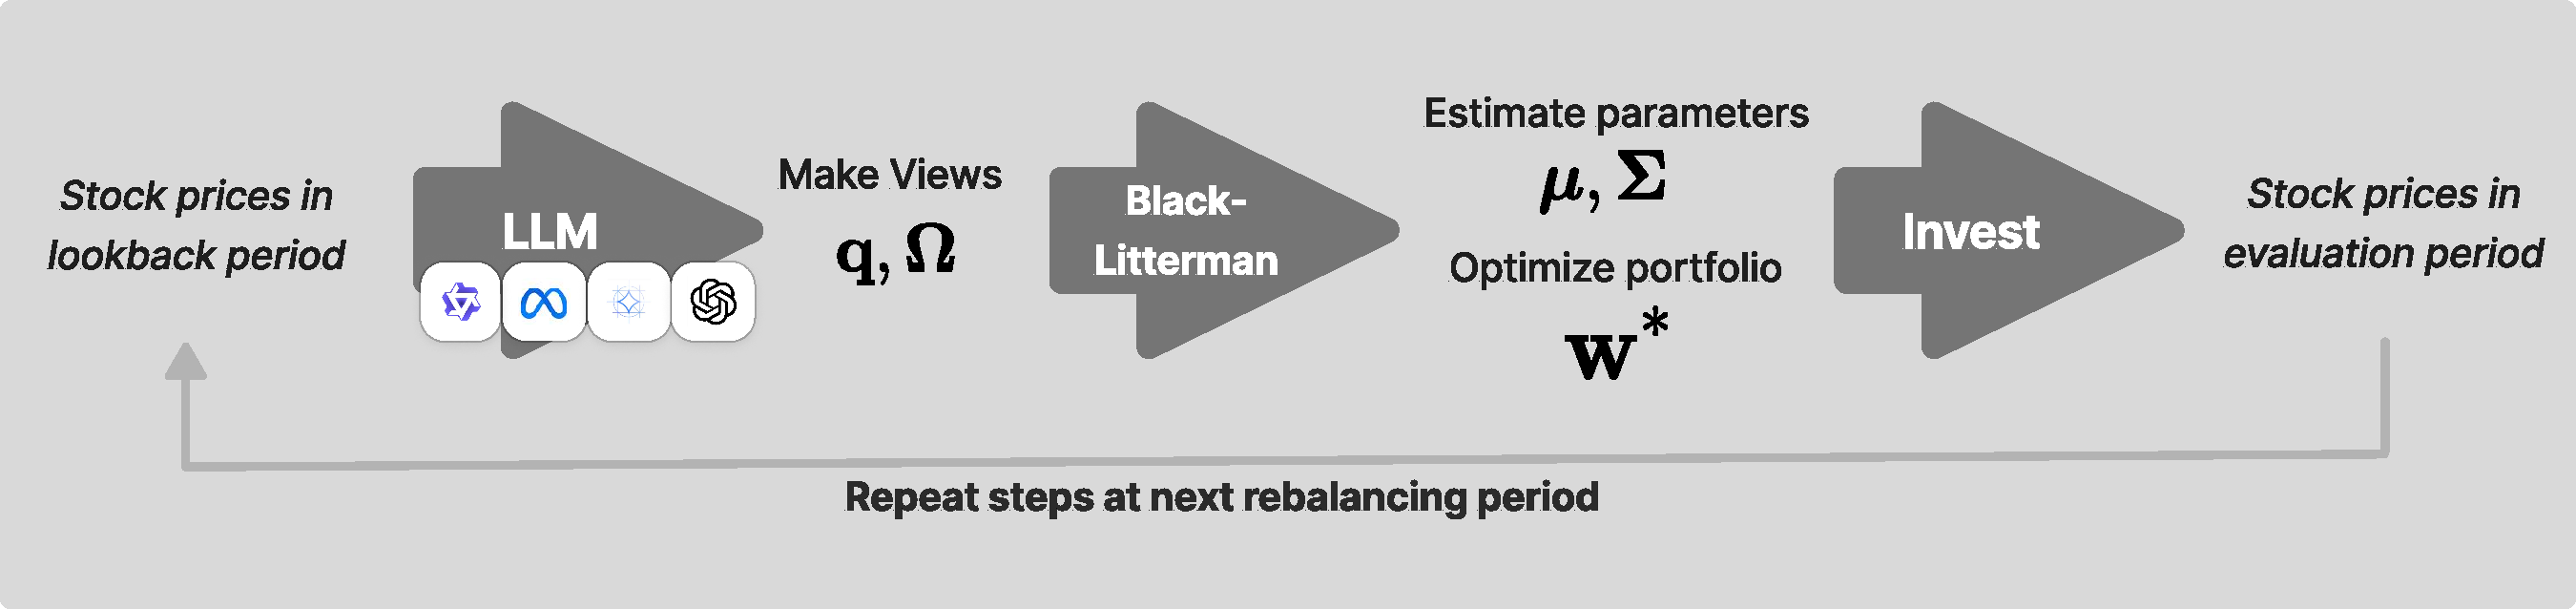
\includegraphics[width=1\linewidth]{figure/model.pdf}
\caption{\textbf{Workflow for mapping LLM predictive distributions into Black-Litterman views.} At decision time $t$, $N$ stochastic LLM forecasts of $h$‑day excess returns yield $\mathbf{q}_t$ and $\mathbf{\Omega}_t$, which combine with the equilibrium prior to form posterior expected returns used for portfolio optimization.}
\label{fig:model}
\end{figure*}

\subsection{A Framework for Prompt‑based Black–Litterman Views}
\textbf{Setup} Fix a decision time $t$ and $n$ assets. Let $h$ denote the forecast horizon, and let $\mathbf{r}_{t:t+h}\in\mathbb{R}^n$ be the vector of $h$‑day excess returns. Under a fixed prompt $\mathcal{P}$ and a fixed model state $\mathcal{S}_t$, the LLM acts as a stochastic forecast generator. For each asset $i$, the model induces a predictive distribution
\begin{equation}
    \tilde{Q}_{i, t} \sim F_{i, t}\left(\cdot \mid \mathcal{P}, \mathcal{S}_t\right)
\end{equation}
where a query samples $\tilde{Q}_{i,t}$ via internal randomness. We issue $N$ queries with $(\mathcal{P},\mathcal{S}_t)$ held fixed and obtain draws $\{\tilde{q}^{(j)}_{i,t}\}_{j=1}^N$. To elicit quantitative views, we use a two‑part prompt. The system prompt instructs the model to output a single scalar representing the $h$‑day expected excess return (in decimals) for a specified ticker, under a fixed output schema that rejects non‑numeric text. The user prompt provides only information timestamped $\le t$: (i) the asset’s recent return series, (ii) sector and market benchmark returns over the same window, and (iii) static metadata (ticker, name, GICS sector/sub‑industry). Section~\ref{appendix:prompts} lists the exact prompts and schema.

\textbf{Estimators} For asset $i$ at time $t$, let
\begin{equation}
    \hat{q}_{i, t}=\frac{1}{N} \sum_{j=1}^N \tilde{q}_{i, t}^{(j)}, \quad \hat{\sigma}_{i, t}^2=\frac{1}{N-1} \sum_{j=1}^N\left(\tilde{q}_{i, t}^{(j)}-\hat{q}_{i, t}\right)^2.
\end{equation}
We interpret $\hat{\sigma}^2_{i,t}$ as the variance of the predictive distribution, not the variance of the sample mean, so it is not divided by $N$. In implementation we apply a small variance floor $\varepsilon>0$ to avoid numerical singularity.



\textbf{Assembling views} We aggregate the individual estimates into the view vector $\mathbf{q}_t=(\hat{q}_{1,t},\ldots,\hat{q}_{n,t})'$ and the diagonal covariance matrix $\mathbf{\Omega}_t=\mathrm{diag}(\hat{\sigma}^2_{1,t},\ldots,\hat{\sigma}^2_{n,t})$. 
Because we generate forecasts asset‑by‑asset, $\mathbf{\Omega}_t$ is diagonal. So, a joint‑view extension would estimate the full covariance from simultaneous multi‑asset draws.
To utilize these inputs in the Black–Litterman framework, we must also specify the picking matrix $\mathbf{P}$, which maps each view to the underlying assets in the portfolio. Since our methodology generates a direct absolute return forecast for every asset in the universe (1-to-1 mapping), we define $\mathbf{P}$ as the $n \times n$ identity matrix ($\mathbf{P}=\mathbf{I}_n$).
This structure implies that the $i$-th view corresponds exclusively to the $i$-th asset (i.e., $P_{ii}=1$ and $P_{ij}=0$ for $i \neq j$), treating each forecast as an absolute view.
Consequently, the estimation provides a complete set of inputs $(\mathbf{q}_t, \mathbf{\Omega}_t, \mathbf{P})$ required for the posterior update in Equation (\ref{eq:BlackLitterman}).

\subsection{Prompt Design Details} \label{appendix:prompts}

To clarify the temporal context for the return prediction task, we include an explicit reference date in the system prompt (Figure~\ref{fig:system_prompt}). This date represents the point in time at which the LLM is expected to provide its analysis—positioned between the past time series data and the future return period. By anchoring the prediction task to a specific date, we help the model better interpret the directionality of the input data and generate temporally coherent forecasts.

To ensure consistent and parseable responses from the LLMs, we adopt a structured output format using the JSON schema supported by the chat completions API endpoint. This approach standardizes the outputs across all LLMs and ensures that each model provides consistently structured responses across repeated queries, reducing the likelihood of formatting errors and facilitating reliable downstream processing.

To enhance the models' numerical sensitivity, all daily return inputs are scaled by 100 (i.e., presented in percentage terms) in the user prompt (Figure~\ref{fig:user_prompt}). For instance, a daily return of -0.0036 is provided as -0.36. This scaling prevents issues arising from the small magnitude of raw daily returns, which can be difficult for LLMs to differentiate and process effectively. This approach is analogous to using basis points in finance to handle small numerical values. By providing a rich, multi-faceted data context and clear instructions, the prompts enable the LLMs to generate informed, quantitative views for portfolio construction.

\begin{figure}[htbp]
\centering
    \scalebox{0.92}{%
    \begin{tcolorbox}[colframe=blue!80!black, colback=blue!10!white, coltitle=white, title=System Prompt, width=1.08\columnwidth]
    \scriptsize
    \setlength{\itemsep}{1pt}%
    \setlength{\topsep}{2pt}%
    \setlength{\partopsep}{0pt}%
    \setlength{\parsep}{0pt}%
    You are providing analysis on \texttt{{\{\{DATE\}\}}}. Predict the average daily return for the next two weeks based on the information provided about a stock's past performance.
    You will receive the following inputs:
    \begin{itemize}
        \item \textbf{Daily Returns}: The stock's daily returns, a time-series from the past two weeks.
        \item \textbf{Company Sector}: The company's GICS sector classification.
        \item \textbf{Sector Returns}: The company sector's daily returns, a time-series from the past two weeks.
        \item \textbf{Market Returns}: The S\&P 500's daily returns, a time-series from the past two weeks.
        \item \textbf{Company Information}:
            \begin{itemize}
                \item Ticker: The stock symbol.
                \item Company Name: The name of the company.
                \item GICS Sector: The Global Industry Classification Standard sector.
                \item GICS Sub-Industry: The sub-industry classification.
            \end{itemize}
    \end{itemize}
    
    \# Steps
    \begin{enumerate}
        \item \textbf{Analyze the Time-Series Data}: Review the historical daily returns to identify patterns, trends, or anomalies that may affect future performance.
        \item \textbf{Consider Sector Performance}: Analyze how the market and the sector's performance might influence the stock's future returns.
        \item \textbf{Incorporate Company Information}: Use the details from the GICS sector and sub-industry, along with the company symbol and name, to contextualize the predicted performance within its industry.
        \item \textbf{Predict Future Returns}: Estimate the average daily returns for the next two weeks based on the analysis of available data.
    \end{enumerate}
    
    \# Output Format
    \begin{quote}
    Return a single float value that represents the predicted average daily return for the stock over the next two weeks, without any additional commentary or explanation.
    \end{quote}
    
    \# Notes
    \begin{itemize}
        \item Ensure the prediction considers the quantified data from the time-series.
        \item Make calculations based on statistical trends from daily returns data.
        \item Pay attention to the trends within both the stock's daily returns and the market's return data.
        \item Consider the relevance of the company's sector to refine your predictions.
        \item Make calculations without additional interpretation or commentary.
    \end{itemize}
    
    \end{tcolorbox}%
    }
    \caption{The structure of the system prompt used to elicit return forecasts from the LLMs.}
    \label{fig:system_prompt}
\end{figure}



 % \label{fig:system_prompt}

\begin{figure}[htbp]
\centering
    \scalebox{0.92}{%
    \begin{tcolorbox}[colframe=green!60!black, colback=green!5!white, coltitle=white, title=User Prompt, width=1.08\columnwidth]
    \scriptsize
    \ttfamily % Use a typewriter font for code-like text
    \textbf{Daily Returns:} [-1.17, -0.92, -2.31, -0.36, -3.02, 2.53, 0.1, -0.23, 0.45]
    
    \vspace{0.5mm}
    \textbf{Company Sector:} Information Technology
    
    \vspace{0.5mm}
    \textbf{Sector Returns:} [-0.14, -0.38, -1.88, 0.03, -1.1, 2.38, -0.41, 0.17, -0.31]
    
    \vspace{0.5mm}
    \textbf{Market Returns:} [0.09, -0.39, -1.61, -0.04, -0.67, 2.05, -0.56, 0.4, -0.01]
    
    \vspace{0.5mm}
    \textbf{Company Information:}
    
    \hspace{5mm} \textbf{Ticker:} AAPL
    
    \hspace{5mm} \textbf{Company Name:} Apple Inc.
    
    \hspace{5mm} \textbf{GICS sector:} Information Technology
    
    \hspace{5mm}     \textbf{GICS sub-industry:} Technology Hardware, Storage \& Peripherals
    
    \end{tcolorbox}%
    }
    \caption{An example user prompt providing data for Apple Inc. (AAPL) on a specific rebalancing date.}
    \label{fig:user_prompt}
\end{figure} % \label{fig:user_prompt}

\subsection{Integrating LLM views into the Black–Litterman model} 
Let $\boldsymbol{\Pi}_t=\delta_t\,\boldsymbol{\Sigma}_t\,\mathbf{w}_{m,t}$ denote the equilibrium $h$-day excess returns implied by the market portfolio $\mathbf{w}_{m,t}$, where $\delta_t>0$ is the representative risk‑aversion scalar, $\boldsymbol{\Sigma}_t$ is the $h$‑day covariance of excess returns estimated from a trailing window, and $m$ indexes the $m$-th asset out of a total of $n$ assets ($m=1,\ldots,n$). Let $\tau>0$ scale prior uncertainty. For picking matrix $\mathbf{P}$, views $\mathbf{q}_t$, and view confidence $\mathbf{\Omega}_t$, the posterior mean of the Black–Litterman model (BLM) is
\begin{equation} \label{eq:BlackLitterman}
    \boldsymbol{\mu}_{\text{BLM}, t}=\left[\left(\tau \boldsymbol{\Sigma}_t\right)^{-1}+\mathbf{P}^{\top} \boldsymbol{\Omega}_t^{-1} \mathbf{P}\right]^{-1}\left[\left(\tau \boldsymbol{\Sigma}_t\right)^{-1} \mathbf{\Pi}_t+\mathbf{P}^{\top} \boldsymbol{\Omega}_t^{-1} \mathbf{q}_t\right].
\end{equation}

We estimate $\delta_t$ as the market price of risk at the $h$-day horizon—computed over the same window as $\boldsymbol{\Sigma}_t$. That is, 
\begin{equation}
    \delta_t = \frac{\widehat{\mathbb{E}}\left[r_{m,t:t+h}^{\text{ex}}\right]}{\widehat{\mathrm{Var}}\left(r_{m,t:t+h}^{\text{ex}}\right)}
\end{equation}
We treat $\tau$ as an ex‑ante hyperparameter and apply standard regularization to ensure numerical stability.
%We calibrate $\delta_t$ by matching the market Sharpe ratio over the estimation window and treat $\tau$ as an ex‑ante hyperparameter. Matrices are regularized to ensure numerical invertibility.

We implement a fixed‑interval rebalancing scheme with horizon $h$. At each decision time $t$: (i) we construct the information set using a rolling lookback window, (ii) elicit $N$ stochastic LLM forecasts to form $(\mathbf{q}_t,\mathbf{\Omega}_t)$, (iii) compute $\boldsymbol{\Pi}_t$ and $\boldsymbol{\Sigma}_t$ at the same horizon $h$, (iv) obtain $\boldsymbol{\mu}_{\text{BLM},t}$ from the BLM update, and (v) solve a mean–variance program
\begin{equation}
    \min _{\mathbf{w}} \lambda \mathbf{w}^{\top} \boldsymbol{\Sigma}_t \mathbf{w} - \mathbf{w}^{\top} \boldsymbol{\mu}_{\text{BLM}, t} \quad \text { s.t. } \quad \mathbf{1}^{\top} \mathbf{w}=1, \mathbf{w} \in \mathcal{C},
\end{equation}
where $\lambda$ is risk aversion and $\mathcal{C}$ encodes portfolio constraints. We hold $\mathbf{w}_t$ for $h$ days and repeat.